\documentclass{template}

\project{machine learning final project}
\title{Classifying and Clustering images based on their authenticity (real or artificial)}
\author{Fardin Abbasi 810199456\\\vspace{0.1cm} Mansour davoudi 810199567\\\vspace{0.1cm} Arash Mohamadpour 810197636\\\vspace{0.1cm} Amirhossein safari 810101213}
\department{\href{https://ece.ut.ac.ir/en/ece}{School of Electrical and Computer Engineering}}
%\abst{Put your abstract here.}


\begin{document}

\chapter{Introduction}\label{ch:in}
\fontsize{13}{15}\selectfont
In recent years, there has been a great focus on generating fake images using artificial intelligence algorithms. One of the well-known algorithms is the Generative Adversarial Network (GAN). A generative adversarial network is a class of machine learning frameworks in which two neural networks compete with each other in a zero-sum game, where one agent's gain is another agent's loss.\\\\
The final goal of this project is to classify fake images from real ones. Like a real-world project, we need to collect the raw dataset and then perform data cleansing and preprocessing. Before diving into the code, it is important to analyze the dataset to gain a good understanding of its behavior.\\\\
Now, let's take a look at how fake image generators like Dall-E and stable diffusion work. These types of generative AI are powered by a computer program called a diffusion model. In simple terms, a diffusion model destroys and recreates images to find statistical patterns within them.\\\\ 
Empirical results demonstrate that fake images generated by various models can be distinguished from real ones, as there exists a common artifact shared by fake images from different models. Fake photos can be effectively attributed to their source models, as different models leave unique fingerprints in their generated images.\cite{gulawani2006cfd}
\\\\At first glance, the project can be divided into 4 parts:
\begin{enumerate}
  \item Data Collection
  \item Data Preparation
    \begin{enumerate}
      \item Feature Extraction
      \item Preprocessing
      \item Dimension Reduction
    \end{enumerate}
  \item Classifying
  \item Clustering
\end{enumerate}

\newpage
%\section{Problem statement}
%\newpage

%\section{Aim and objectives}





%Now I am going to cross-reference the figure by using its label \Cref{fig:logo}.

%\begin{table}
%\caption{4}
%\label{tab:city}
%\entries{
%person  & singEnglish & singGaeilge & pluralEnglish & pluralGaeilge\\
%    1st & at me       & agam        & at us         & againn\\
%    2st & agat        & at you      & agaibh        & other \\ 
%    3rd & at him      & aige        & at them       & acu\\
%        & at her      & aici        &               &\\
%}
%\end{table}

%Let's cross-reference to \Cref{tab:city}.

    

\chapter{Data Preparation}\label{ch:lr}
\section{Feature Extraction}
In this project, besides the given deep features that are likely extracted from a CNN, we need to extract handcrafted features. Handcrafted features are features that are manually engineered by the data scientist.\\\\
The approach involved using two common techniques, namely Local Binary Patterns (LBP) and Fast Fourier Transform (FFT).\\\\
LBP is a texture descriptor technique that characterizes the local structure of an image by comparing the intensity of a central pixel with its surrounding neighbors. By applying LBP, the project aimed to capture relevant textural details that could contribute to the understanding and classification of the images or data.\\\\
FFT transforms a signal from the time domain to the frequency domain, enabling the identification of different frequency components within the signal. By using FFT, we extracted frequency-based features that could provide insights into the underlying patterns or characteristics of the data.\\\\
After applying LBP and FFT individually, the next step involved concatenating the extracted features. This process combined the information captured by both techniques, creating a more comprehensive feature representation. Subsequently, PCA was applied to reduce the dimensionality of the concatenated features. PCA aimed to identify the most significant patterns and reduce the feature space, allowing for efficient data analysis and potential improvement in subsequent tasks such as classification or clustering.
\section{Preprocessing}
Data preprocessing is an integral step in machine learning, as the quality of the data and the useful information that can be derived from it directly affect the ability of our model to learn. Therefore, it is necessary to preprocess our data before feeding it into our model.
\newpage
.\\
In this project, the dataset has been preprocessed as below:
\begin{enumerate}[label=\roman*.]
  \item Handling Null Values: In any real-world dataset, there are always a few null values.
  \item Data Cleansing: Data cleansing is the process of identifying and correcting corrupt or inaccurate records in a dataset. It involves detecting incomplete, incorrect, inaccurate, or irrelevant parts of the data and then taking actions such as replacing, modifying, or deleting the problematic data. For instance:
  \begin{enumerate}[label=\alph*.]
    \item There are a few incorrect labels, such as "forest" or "Jungle" instead of "jungle," "DALL.E," and other derivatives instead of "DALL-E."
    \item Removing irrelevant parts of labels, including image 
    formats and student IDs
  \end{enumerate}
  \item Standardization: In Standardization, we transform our values such that the mean of the values is 0 and the standard deviation is 1.
  \item Test, Train {\&}  Validation Split: Train data is used for training the model, validation data is used for tuning hyperparameters and choosing the best model, and test data is used for evaluating the chosen model.
\end{enumerate}
\begin{figure}
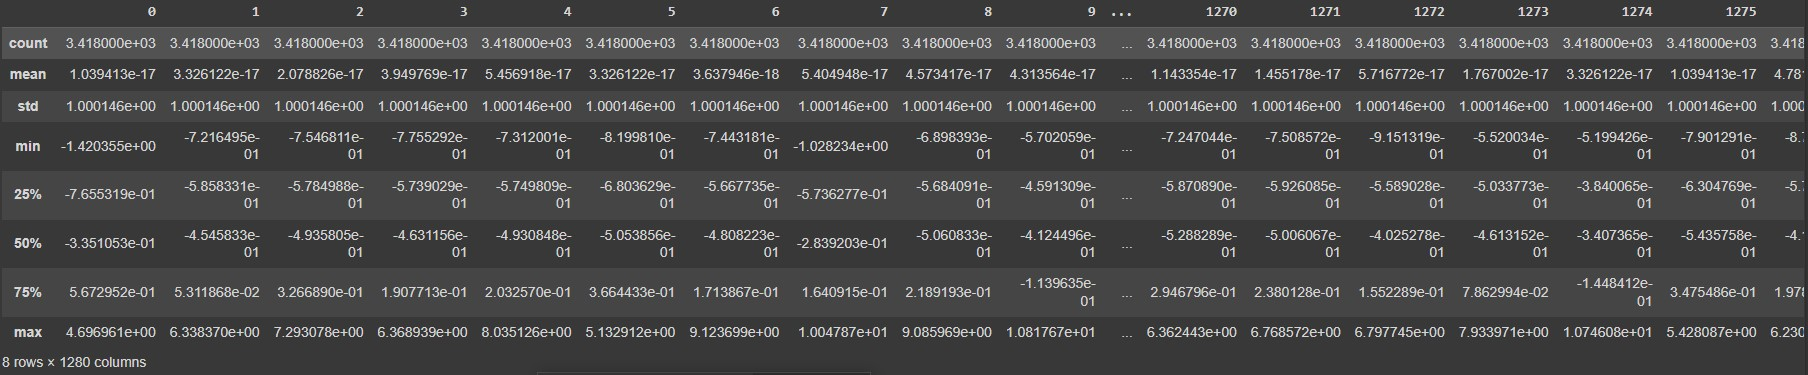
\includegraphics[scale=0.33]{preprocessing.jpg}
\caption{}
\label{fig:logo}
\end{figure}
As you see, features are transformed such that the mean of each feature is 0 and the standard deviation is 1.\\\\
Labels Summary:
\begin{figure}
  \centering
  \begin{subfigure}{0.3\textwidth}
    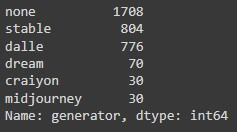
\includegraphics[width=\linewidth]{preprocessing1.jpg}
    \caption{}
    \label{fig:image1}
  \end{subfigure}
  \begin{subfigure}{0.3\textwidth}
    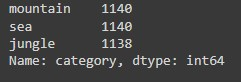
\includegraphics[width=\linewidth]{preprocessing2.jpg}
    \caption{}
    \label{fig:image2}
  \end{subfigure}
  \begin{subfigure}{0.3\textwidth}
    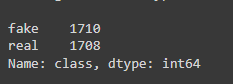
\includegraphics[width=\linewidth]{preprocessing3.jpg.png}
    \caption{}
    \label{fig:image3}
  \end{subfigure}
  \caption{Labels Summary}
  \label{fig:three_images}
\end{figure}
\newpage
\section{Dimension Reduction}
Dimension reduction is a fundamental technique in data analysis and machine learning. Its goal is to reduce the number of variables or features in a dataset while preserving the essential information. This technique is especially valuable when working with high-dimensional data, as it helps address challenges related to visualization, computational efficiency, and interpretability.
\\\\
\textbf{Significance of Dimension Reduction:}
\begin{enumerate}
  \item Simplification of Data: High-dimensional datasets can be complex and difficult to analyze. Dimension reduction helps simplify the data representation by reducing the number of variables, making it easier to understand and interpret.
  \item Visualization: Dimension reduction techniques allow us to visualize data in lower-dimensional spaces, such as 2D or 3D, facilitating a better understanding of patterns and relationships among the data points.
  \item Noise Reduction: By eliminating irrelevant or redundant features, dimension reduction can help reduce the impact of noise or irrelevant data, improving the quality of subsequent analyses or machine learning models.
  \item Computational Efficiency: High-dimensional data often requires significant computational resources. By reducing the dimensionality, the computational complexity can be reduced, resulting in faster processing and analysis.
\end{enumerate}
In this project we use the PCA and LOL techniques to reduce dimension.\\\\
\textbf{Linear Optimal Low-Rank Projection (LOL):}\\
The key intuition behind LOL is that we can jointly use the means and variances from each class (like LDA and CCA), but without requiring more dimensions than samples (like PCA), or restrictive sparsity assumptions. Using random matrix theory, we are able to prove that when the data are sampled from a Gaussian, LOL finds a better low-dimensional representation than PCA, LDA, CCA, and other linear methods.\\\\
\textbf{Principal Component Analysis (PCA):}\\
PCA is a widely used technique for dimension reduction. It identifies a new set of variables, called principal components, that are linear combinations of the original features. These components are ordered in terms of the amount of variance they explain in the data.
\begin{figure}
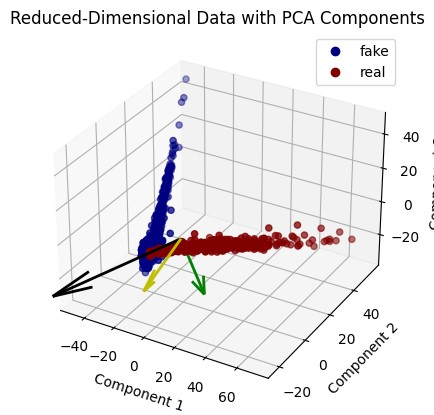
\includegraphics[scale=1]{pca.jpg}
\caption{}
\label{fig:logo}
\end{figure}
\chapter{Classification}\label{ch:me}

Classification is a supervised machine learning method where the model aims to predict the correct label of a given input data. In classification, the model is trained using the training data and then evaluated on test data before being used to make predictions on new unseen data.
\\
There are several methods for classification, and each is preferred based on different circumstances, such as the distribution and size of the dataset. In this project, we will test several popular methods to assess their performance.
\\
\begin{figure}
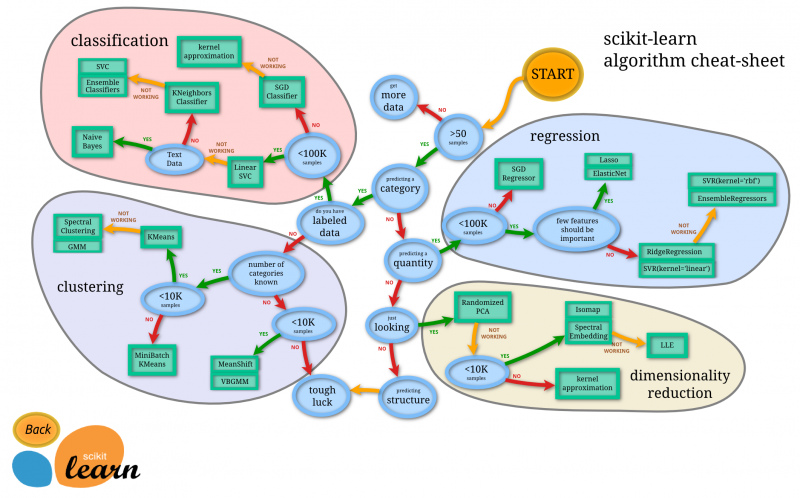
\includegraphics[scale=0.5]{ML_map.jpg}
\caption{scikit-learn algorithm cheat sheet}
\label{fig:logo}
\end{figure}
\section{Logistic Regression}
Logistic regression is a classification algorithm used to determine the probability of event success and event failure. It is employed when the dependent variable is binary (0/1, True/False, Yes/No) in nature. Logistic regression categorizes data into discrete classes by analyzing the relationship within a labeled dataset. It learns a linear relationship from the provided dataset and incorporates non-linearity through the use of the Sigmoid function.\cite{LR}\\
\begin{table}[h]
  \begin{center}
    \begin{tabular}[t]{|p{6cm}|p{6cm}|}
    \hline
         \textbf{Advantages} & \textbf{Disadvantages}\\
    \hline  
         Logistic regression is easier to implement, interpret, and very efficient to train. & If the number of observations is lesser than the number of features, Logistic Regression should not be used, otherwise, it may lead to overfitting. \\
    \hline 
         It makes no assumptions about distributions of classes in feature space. & It constructs linear boundaries.  \\
    \hline 
         It can easily extend to multiple classes(multinomial regression) and a natural probabilistic view of class predictions. & The major limitation of Logistic Regression is the assumption of linearity between the dependent variable and the independent variables.  \\
         \hline 
         It not only provides a measure of how appropriate a predictor(coefficient size)is but also its direction of association (positive or negative). & It can only be used to predict discrete functions. Hence, the dependent variable of Logistic Regression is bound to the discrete number set.  \\
         \hline 
         It is very fast at classifying unknown records. & Non-linear problems can’t be solved with logistic regression because it has a linear decision surface. Linearly separable data is rarely found in real-world scenarios.  \\
         \hline 
         Good accuracy for many simple data sets and it performs well when the dataset is linearly separable. & Logistic Regression requires average or no multicollinearity between independent variables.  \\
         \hline 
        It can interpret model coefficients as indicators of feature importance. & It is tough to obtain complex relationships using logistic regression. More powerful and compact algorithms such as Neural Networks can easily outperform this algorithm. \\
         \hline 
        high-dimensional datasets. One may consider Regularization (L1 and L2) techniques to avoid over-fitting in these scenarios. & But Logistic Regression needs that independent variables are linearly related to the log odds (log(p/(1-p)).  \\
         \hline 
         Logistic regression is less inclined to over-fitting but can overfit  & In Linear Regression, independent and dependent variables are related linearly.  \\
          \hline 
    \end{tabular} 
  \end{center}
\caption{}
\end{table}
\subsection{Evaluation with Deep Features}
For training the model, the "Newton-Cholesky" solver is used, which is recommended when the number of samples is much larger than the number of features.
\\
The classification report and the confusion matrix are shown below, demonstrating the performance of the model:
\begin{figure}
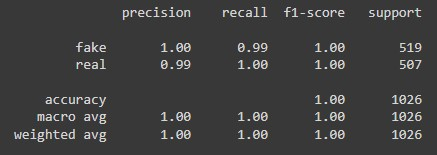
\includegraphics[scale=0.9]{LR1.jpg}
\caption{classification report}
\label{fig:logo}
\end{figure}
\begin{figure}
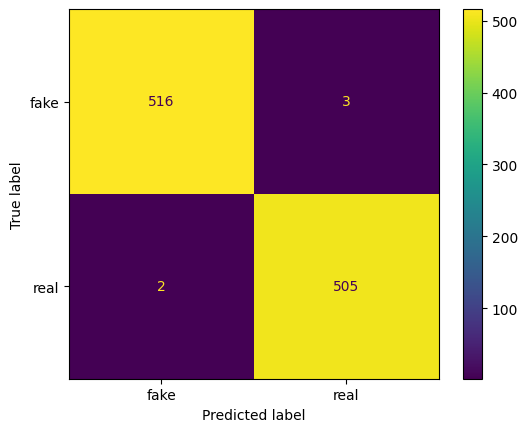
\includegraphics[scale=0.9]{LR2.png}
\caption{Confusion Matrix}
\label{fig:logo}
\end{figure}
\subsection{Evaluation with Handcraft Features}
The classification report and the confusion matrix, shown below, demonstrate that our extracted features do not classify well using Logistic Regression:
\begin{figure}
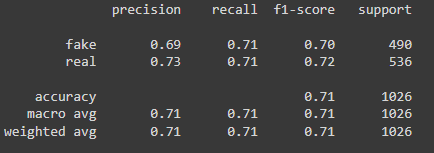
\includegraphics[scale=0.9]{LR3.png}
\caption{classification report}
\label{fig:logo}
\end{figure}
\begin{figure}
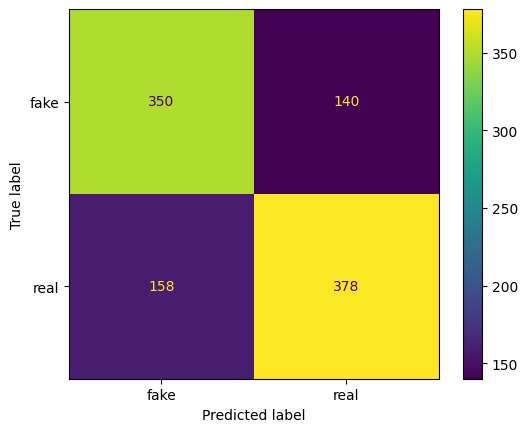
\includegraphics[scale=0.9]{LR4.png}
\caption{Confusion Matrix}
\label{fig:logo}
\end{figure}
\section{SVM}
SVM is a supervised machine learning algorithm that aids in classification or regression problems. Its goal is to find an optimal boundary between the possible outputs.\\
In its simplest form, SVM is applied to binary classification, dividing data points into either 1 or 0.
\newpage
.\\
\textbf{Advantages:}
\begin{itemize}
    \item SVM works relatively well when there is a clear margin of separation between classes.

    \item SVM is more effective in high-dimensional spaces.
    \item SVM is effective in cases where the number of dimensions is greater than the number of samples.
    \item SVM is relatively memory efficient
\end{itemize}
\textbf{Disadvantages:}
\begin{itemize}
    \item The SVM algorithm is not suitable for large data sets.
    \item SVM does not perform very well when the data set has more noise i.e. target classes are overlapping.
    \item In cases where the number of features for each data point exceeds the number of training data samples, the SVM will underperform. 
    \item As the support vector classifier works by putting data points, above and below the classifying hyperplane there is no probabilistic explanation for the classification.\cite{svm}
\end{itemize}
\subsection{Evaluation with Deep Features}
\begin{equation*}
\min_{w, b, \xi} \frac{1}{2}\|w\|^2 + C\sum_{i=1}^{n}\xi_i
\end{equation*}
subject to:
\begin{align*}
& y_i(w^T x_i + b) \geq 1 - \xi_i, \quad i = 1, 2, \ldots, n \\
& \xi_i \geq 0, \quad i = 1, 2, \ldots, n
\end{align*}
C is a parameter which determines the trade-off between lower error or higher margin. In order to choose this hyperparameter, we used grid search technique and the best C equals to 0.1.\\
The classification report and the confusion matrix are shown as below which demonstrate how well the model works:
\begin{figure}
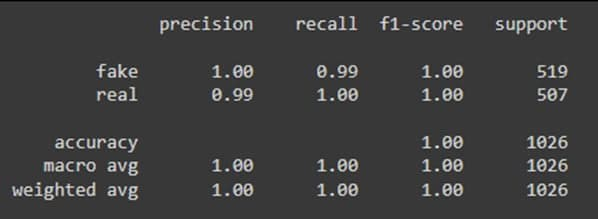
\includegraphics[scale=0.75]{svm1.jpg}
\caption{classification report}
\label{fig:logo}
\end{figure}
\begin{figure}
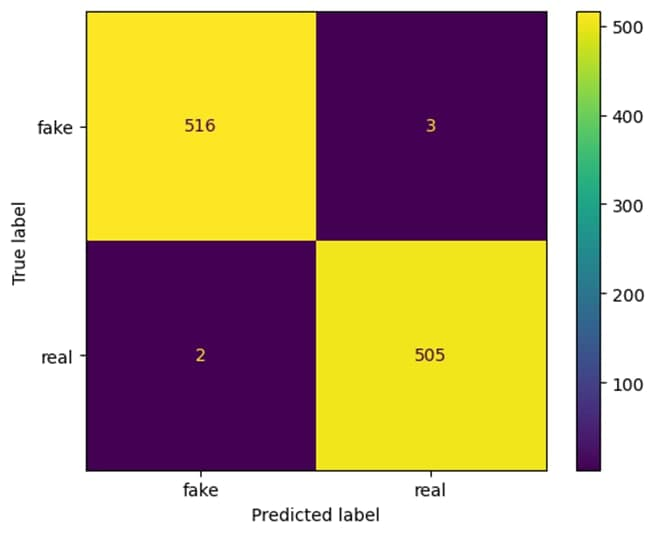
\includegraphics[scale=0.7]{svm2.jpg}
\caption{Confusion Matrix}
\label{fig:logo}
\end{figure}
\subsection{Evaluation with Handcraft Features}
The classification report and confusion matrix shown below demonstrate that this classification incorrectly classifies all the images as "fake" or "real," resulting in poor classification performance:
\begin{figure}
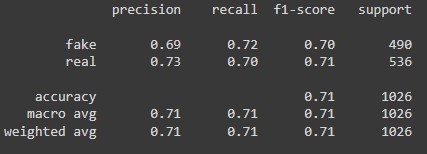
\includegraphics[scale=0.7]{SVM3.jpg}
\caption{classification report}
\label{fig:logo}
\end{figure}
\begin{figure}
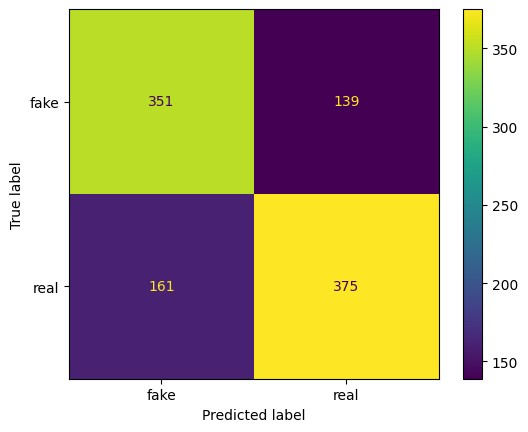
\includegraphics[scale=0.6]{SVM4.jpg}
\caption{Confusion Matrix}
\label{fig:logo}
\end{figure}
\section{Random Forest}
Random forests or random decision forests are an \textbf{ensemble learning} method for classification, regression, and other tasks that operates by constructing a multitude of decision trees at training time. For classification tasks, the output of the random forest is the class selected by most trees. For regression tasks, the mean or average prediction of the individual trees is returned.\cite{rf}
\begin{figure}
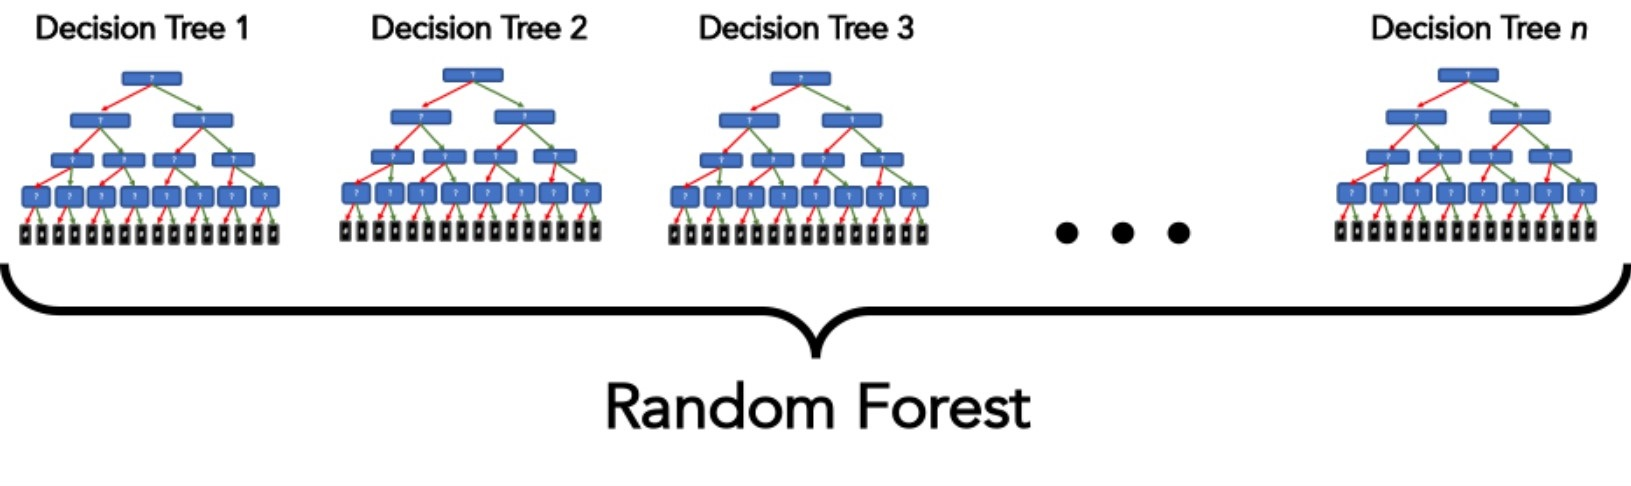
\includegraphics[scale=0.35]{RandF.jpg}
\caption{Random Forest}
\label{fig:logo}
\end{figure}
'\\
\textbf{Random Forest Features:}
    \begin{itemize}
    \item The accuracy of Random forest is generally very high.
    \item Its efficiency is particularly Notable in Large Data sets.
    \item Provides an estimate of important variables in classification. 
    \item Forests Generated can be saved and reused.
    \item Unlike other models, It doesn't overfit with more features.
\end{itemize}
\subsection{Evaluation with Deep Features}
Two importent hyperparameters to find in random forest method, are the number of estimators and the maximum depth. The Best Hyperparameters are found by Randomized Search CV
\begin{verbatim}
     Best Hyperparameters: {'n_estimators': 85, 'max_depth': 100}
\end{verbatim}
The classification report and the confusion matrix are shown as below which demonstrate how well the model works:
\begin{figure}
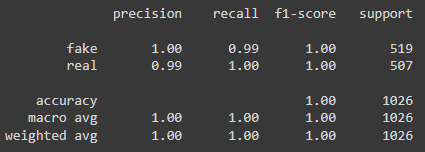
\includegraphics[scale=0.7]{RF1.png}
\caption{classification report}
\label{fig:logo}
\end{figure}
\begin{figure}
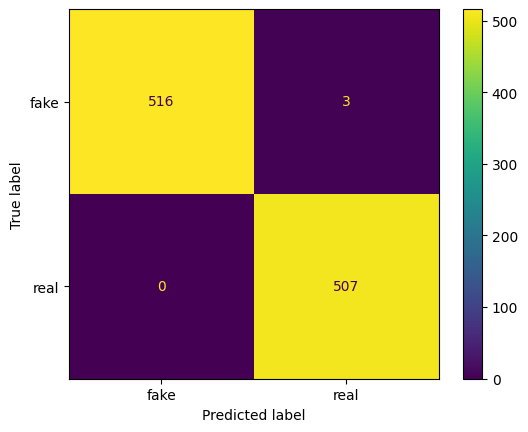
\includegraphics[scale=0.7]{RF2.png}
\caption{ Confusion Matrix}
\label{fig:logo}
\end{figure}
Also the first and second trees are shown as below:
\begin{figure}
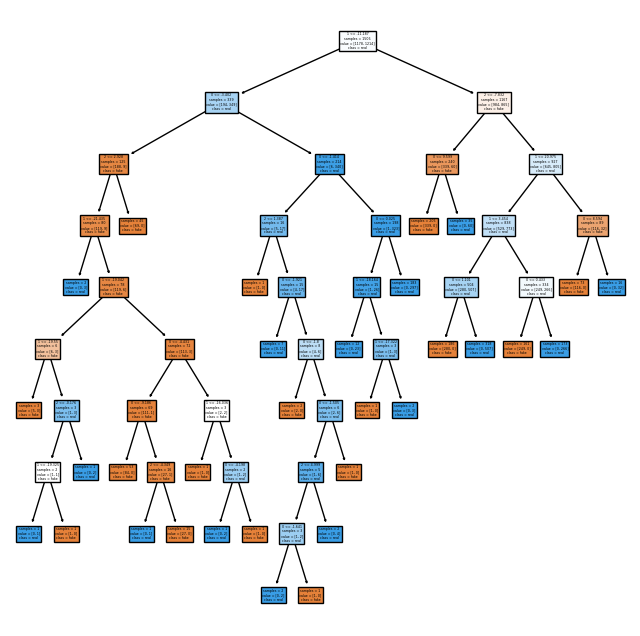
\includegraphics[scale=0.7]{RF3.png}
\caption{}
\label{fig:logo}
\end{figure}
\begin{figure}
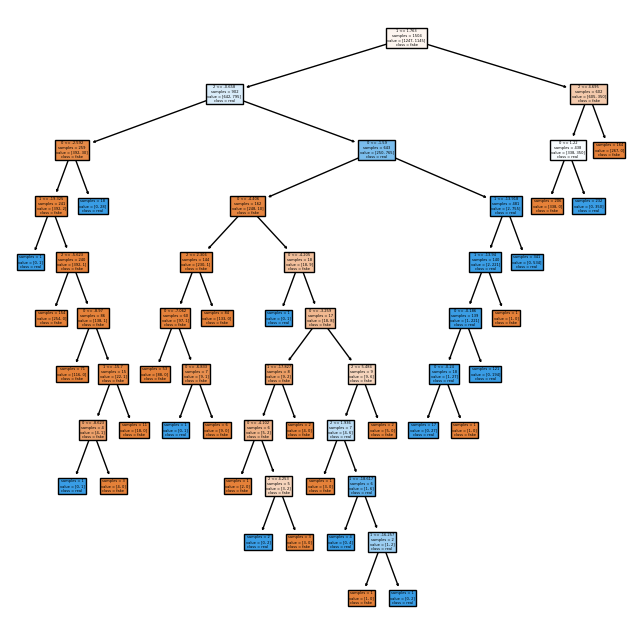
\includegraphics[scale=0.7]{RF4.png}
\caption{}
\label{fig:logo}
\end{figure}
\chapter{Clustering}\label{ch:me}
Clustering is the task of partitioning unlabeled data or data points into different clusters based on their similarities, with the objective of grouping similar data points together while distinguishing them from other groups. In other words, the clustering process aims to identify clusters or groups with similar characteristics and assign data points to these clusters.\\\\
All clustering methods can roughly be divided into four groups:
\begin{enumerate}
  \item Hierarchical clustering
  \item Centroid-based clustering
  \item Graph-based clustering
  \item Density-based clustering
\end{enumerate}
\begin{figure}
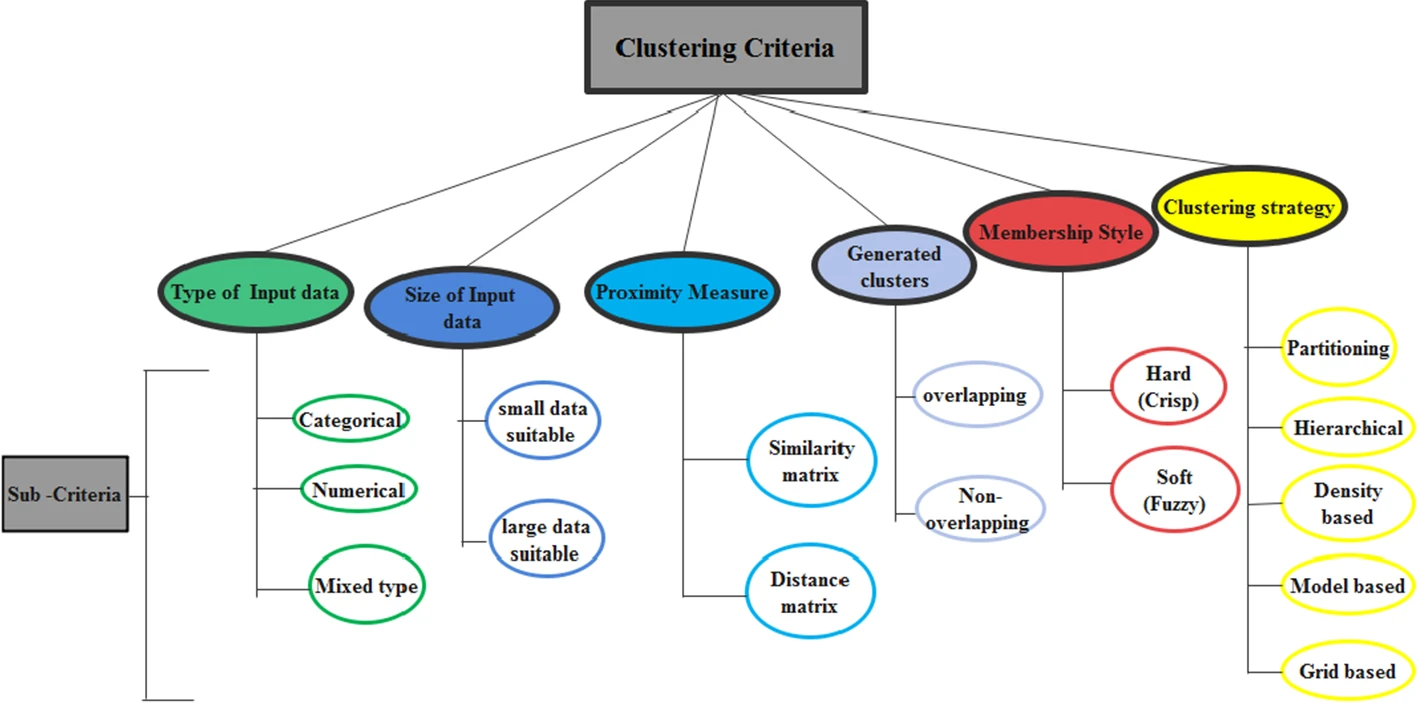
\includegraphics[scale=0.4]{Clustering.png}
\caption{Clustering Criteria}
\label{fig:logo}
\end{figure}
\section{Mini Batch K-Means}
K-means is one of the most popular clustering algorithms, primarily due to its efficient time performance. However, as the size of the datasets being analyzed increases, the computation time of K-means also increases because it requires the entire dataset to be stored in memory. To address this issue, several methods have been proposed to reduce the computational and memory costs of the algorithm. One such approach is the \textbf{Mini-Batch K-means algorithm.}\\
The Mini-Batch K-means algorithm is faster than the traditional batch K-means algorithm but may yield slightly different results due to the use of mini-batches for computations.\cite{CL1}\\\\
\textbf{Pros:}
\begin{enumerate}
  \item Simple: It is easy to implement k-means and identify unknown groups of data from complex data sets. The results are presented easily and simply.
  \item Flexible: K-means algorithm can easily adjust to the changes. If there are any problems, adjusting the cluster segment will allow changes to easily occur in the algorithm.
  \item Suitable in a large dataset: K-means is suitable for a large number of datasets and it’s computed much faster than the smaller dataset. It can also produce higher clusters.
  \item Efficient: The algorithm used is good at segmenting the large data set. Its efficiency depends on the shape of the clusters. K-means works well in hyper-spherical clusters.
  \item Time complexity: K-means segmentation is linear in the number of data objects thus increasing execution time. It doesn’t take more time in classifying similar characteristics in data like hierarchical algorithms.
  \item Computation cost: Compared to using other clustering methods, a k-means clustering technique is fast and efficient in terms of its computational cost O(K*n*d).
  \item Accuracy: K-means analysis improves clustering accuracy and ensures information about a particular problem domain is available. Modification of the k-means algorithm based on this information improves the accuracy of the clusters.
  \item Spherical clusters: This mode of clustering works great when dealing with spherical clusters. It operates with an assumption of joint distributions of features since each cluster is spherical. All the clusters' features or characters have equal variance and each is independent of the other.
\end{enumerate}
\newpage
.\\
\textbf{Cons:}
\begin{enumerate}
  \item No-optimal set of clusters: K-means doesn’t allow the development of an optimal set of clusters and for effective results, you should decide on the clusters before.
  \item Lacks consistency: K-means clustering gives varying results on different runs of an algorithm. A random choice of cluster patterns yields different clustering results resulting in inconsistency.
  \item Uniform effect: It produces clusters with uniform sizes even when the input data has different sizes.
  \item Order of values: How data is ordered in building the algorithm affects the final results of the data set.
  \item Handle numerical data: K-means algorithm can be performed in numerical data only.
  \item Operates in assumption: K-means clustering technique assumes that we deal with spherical clusters and each cluster has equal numbers for observations. The spherical assumptions have to be satisfied. The algorithm can’t work with clusters of unusual size.
  \item Specify K-values: For K-means clustering to be effective, you have to specify the number of clusters (K) at the beginning of the algorithm.
  \item Prediction issues: Predicting the k-values or the number of clusters is difficult. It is also difficult to compare the quality of the produced clusters.\cite{CL2}
\end{enumerate}
Inertia is the sum of the squared distances of samples to their closest cluster center. The goal is to minimize this value. However, if we choose K to be equal to the number of samples, the inertia will be 0. While this is the smallest possible inertia value, it does not achieve our goal of clustering the data into an optimal number of clusters.\\
As the number of clusters increases, the inertia value decreases. Therefore, we need to manually select K while considering the trade-off between the inertia value and the number of clusters. The Elbow Method is commonly used to determine the appropriate value of K. We plot the inertia values against the number of clusters and choose the "elbow point" on the graph. After this point, the improvement in the inertia value becomes less significant, indicating that adding more clusters may not provide significant benefits.
\subsection{Evaluation with Deep Features}
The clustering results for different number of clusters are shown as below:
\begin{figure}
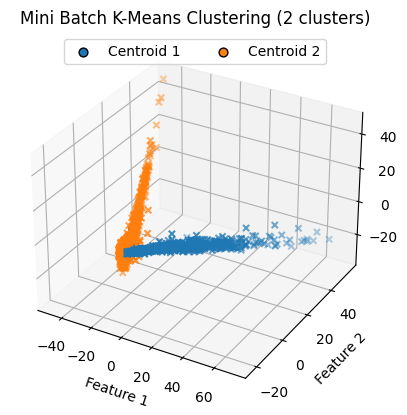
\includegraphics[scale=0.7]{Clustering1.png}
\caption{}
\label{fig:logo}
\end{figure}
\begin{figure}
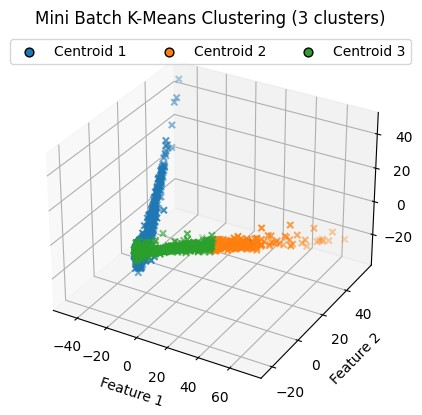
\includegraphics[scale=0.7]{Clustering2.png.jpg}
\caption{}
\label{fig:logo}
\end{figure}
\begin{figure}
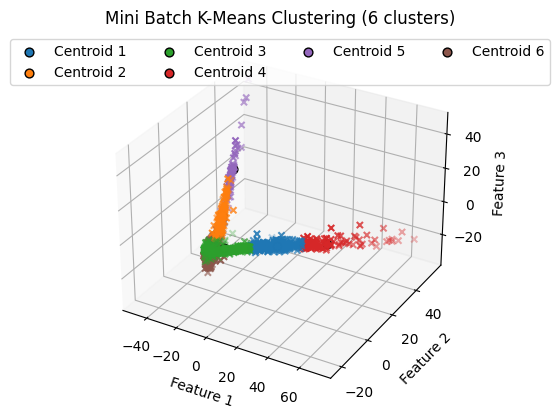
\includegraphics[scale=0.7]{Clustering3.png.jpg.png}
\caption{}
\label{fig:logo}
\end{figure}
\begin{figure}
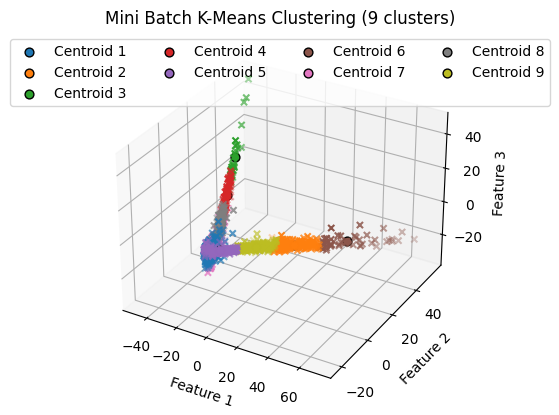
\includegraphics[scale=0.7]{Clustering4.png.jpg.png}
\caption{}
\label{fig:logo}
\end{figure}
\begin{figure}
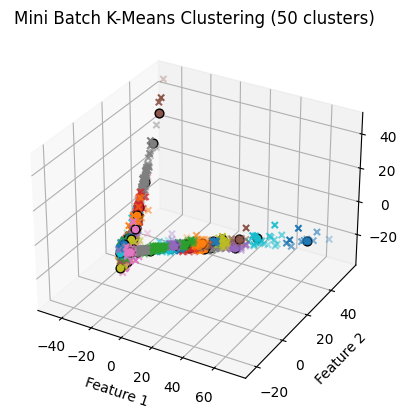
\includegraphics[scale=0.7]{Clustering5.png}
\caption{}
\label{fig:logo}
\end{figure}
The best number of clusters, is elbow point in the plot of inertia with respect to number of clusters:
\begin{figure}
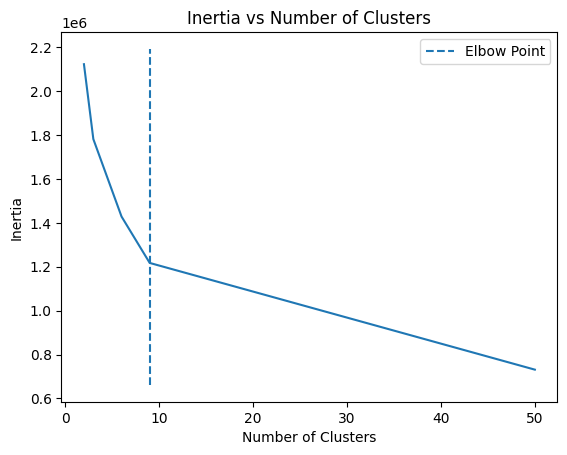
\includegraphics[scale=0.8]{Clustering6.png}
\caption{}
\label{fig:logo}
\end{figure}
\newpage
\subsection{Evaluation with Handcraft Features}
The clustering results for different number of clusters are shown as below:
\begin{figure}
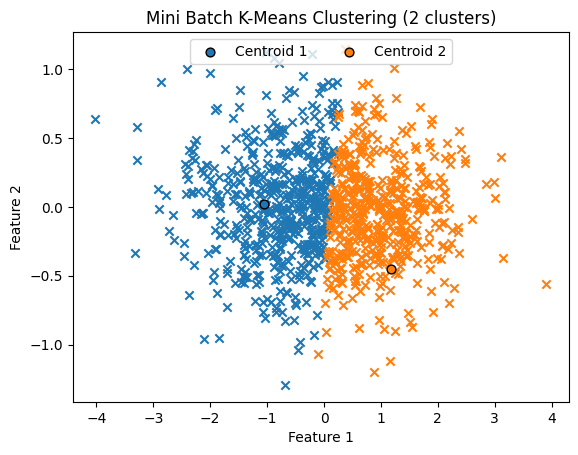
\includegraphics[scale=0.7]{c1.png}
\caption{}
\label{fig:logo}
\end{figure}
\begin{figure}
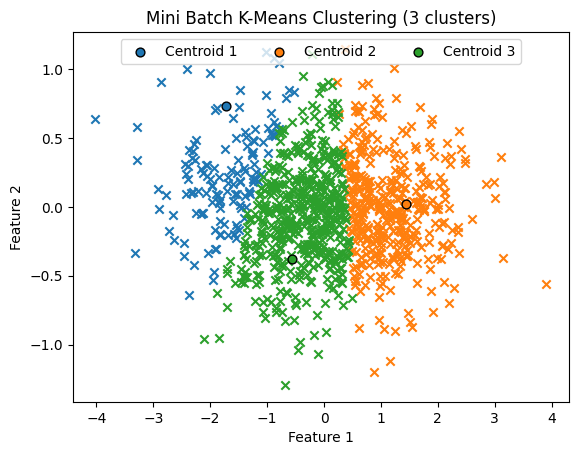
\includegraphics[scale=0.7]{C2.png}
\caption{}
\label{fig:logo}
\end{figure}
\begin{figure}
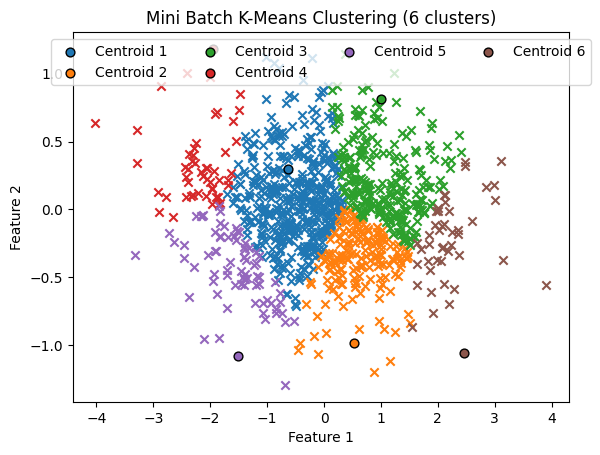
\includegraphics[scale=0.7]{C3.png}
\caption{}
\label{fig:logo}
\end{figure}
\begin{figure}
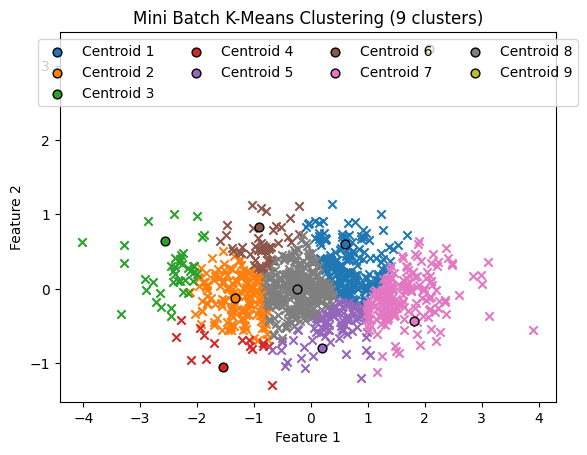
\includegraphics[scale=0.7]{C4.png}
\caption{}
\label{fig:logo}
\end{figure}
\begin{figure}
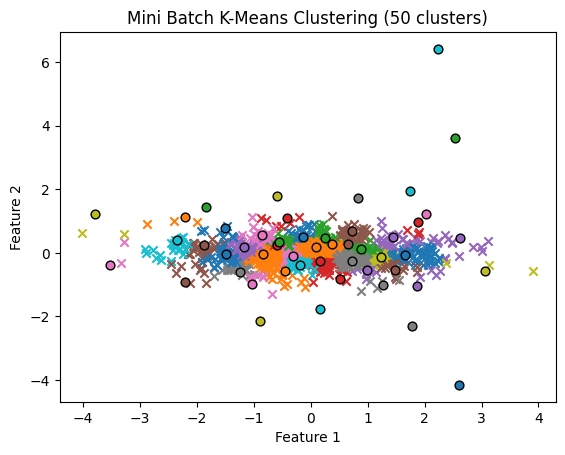
\includegraphics[scale=0.7]{C5.png}
\caption{}
\label{fig:logo}
\end{figure}
The best number of clusters, is elbow point in the plot of inertia with respect to number of clusters:
\begin{figure}
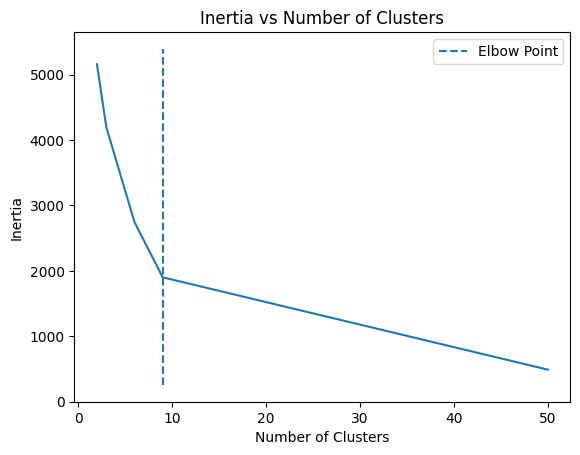
\includegraphics[scale=0.7]{C6.png}
\caption{}
\label{fig:logo}
\end{figure}
\newpage
\section{Gaussian Mixture Models}
Gaussian Mixture Models (GMMs) are powerful probabilistic models used for clustering and density estimation. By combining multiple Gaussian components, GMMs can represent various data patterns and capture the underlying structure of the data. They have widespread applications in clustering, anomaly detection, image and speech recognition, and data generation. With the ability to estimate parameters using the Expectation-Maximization (EM) algorithm, GMMs provide valuable insights and analysis capabilities in diverse fields.\\\\
The Expectation-Maximization (EM) algorithm is commonly employed to estimate the parameters of Gaussian Mixture Models (GMMs), including the mean, covariance, and cluster weights. The EM algorithm iteratively refines these parameters by alternating between the expectation (E) step, where data points are probabilistically assigned to clusters, and the maximization (M) step, where the model parameters are updated based on the assignments.\\\\
\textbf{Advantages: }
    \begin{itemize}
    \item Flexibility: GMMs can identify clusters of various shapes and sizes, making them suitable for datasets with complex distributions and overlapping clusters.
    \item Probabilistic Assignments: Unlike K-means, which yields hard cluster assignments, GMMs provide soft assignments, which are more informative and useful for uncertainty estimation.
    \item Outlier Robustness: GMMs are less sensitive to outliers since data points are assigned probabilities to clusters rather than being hard-assigned.
    \item Model Selection: GMMs offer a natural framework for model selection using techniques like the Bayesian Information Criterion (BIC) or cross-validation
\end{itemize}
\textbf{Limitations and Disadvantages:}
    \begin{itemize}
    \item Computationally More Demanding: Compared to K-means, GMMs are computationally more demanding due to the iterative EM algorithm, making them less efficient for large datasets.
    \item Initialization Sensitivity: GMMs are sensitive to initialization, and suboptimal initializations may lead to convergence to local optima.
\end{itemize}
Gaussian Mixture Models vs. K-means:\\
K-means, as mentioned in the introduction, is widely used due to its efficient time performance. However, it suffers from scalability issues when dealing with large datasets.\\
Gaussian Mixture Models tackle the limitations of K-means. Instead of assigning a data point exclusively to a single cluster, GMMs assign probabilities to data points belonging to each cluster. This makes GMMs more suitable for datasets with complex structures, overlapping clusters, or uncertain data points.\\

For finding the optimal number of components in a cluster, the Akaike Information Criterion (AIC) and Bayesian Information Criterion (BIC) are commonly used measures.\\
AIC is a statistical measure that quantifies the quality of a model relative to the number of parameters it uses. It balances the goodness of fit of the model with the complexity of the model. When comparing different models, the model with the lowest AIC is preferred.\\
BIC is another criterion used for model selection. Like the AIC, it also penalizes models for their complexity. However, the BIC applies a stronger penalty for model complexity compared to the AIC. When comparing different models, the model with the lowest BIC is preferred.\\
Both the AIC and BIC are useful tools in model selection and determining the optimal number of components in a cluster.\\\\
\subsection{Evaluation with Deep Features}
\begin{figure}
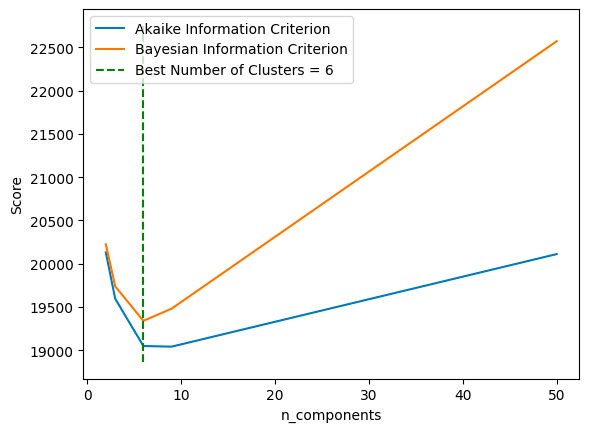
\includegraphics[scale=0.5]{m1.png}
\caption{AIC and BIC }
\label{fig:logo}
\end{figure}
\subsection{Evaluation with Handcraft Features}
\begin{figure}
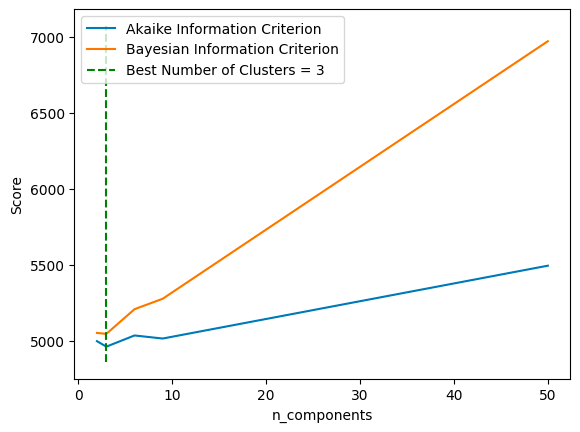
\includegraphics[scale=0.5]{m2.png}
\caption{AIC and BIC}
\label{fig:logo}
\end{figure}
\end{document}
\end{document}

\section{Random Forest}
Random forests or random decision forests are an \textbf{ensemble learning} method for classification, regression, and other tasks that operates by constructing a multitude of decision trees at training time. For classification tasks, the output of the random forest is the class selected by most trees. For regression tasks, the mean or average prediction of the individual trees is returned.
\\
\begin{figure}
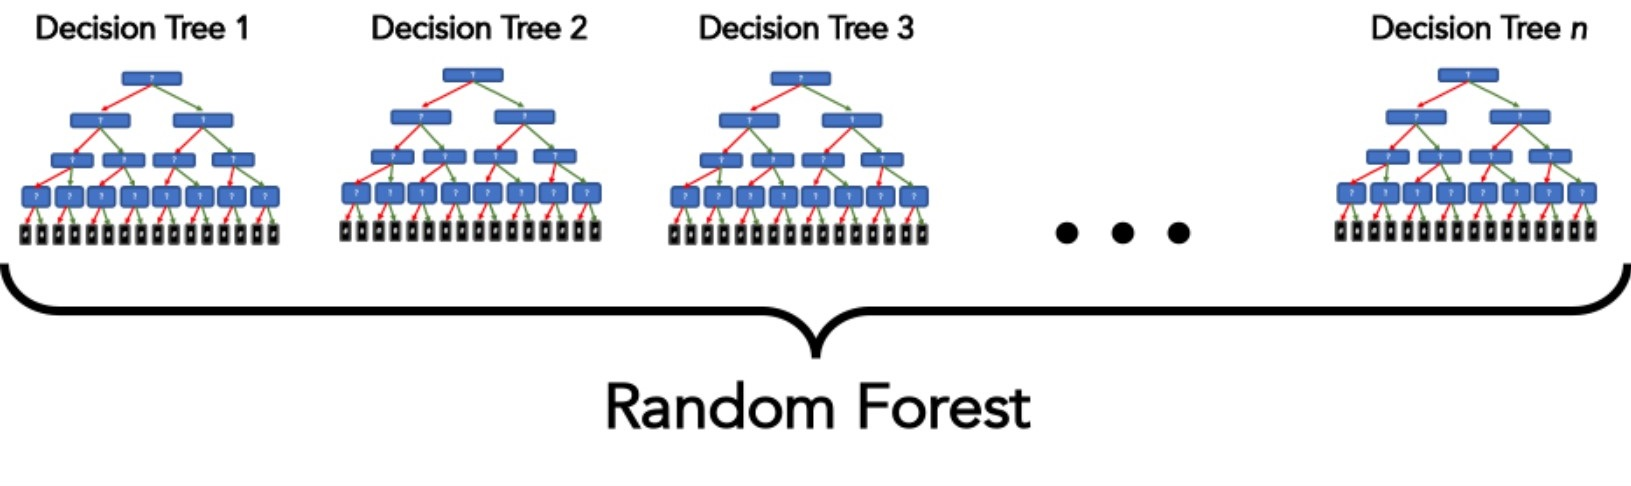
\includegraphics[scale=0.35]{RandF.jpg}
\caption{Put your caption here.}
\label{fig:logo}
\end{figure}
\newpage
.\\
\textbf{Random Forest:}
\begin{itemize}
    \item The accuracy of Random forest is generally very high
    \item Its efficiency is particularly Notable in Large Data sets.
    \item Provides an estimate of important variables in classification
    \item SVM is relatively memory efficient
    \item Unlike other models, It doesn't overfit with more features
\end{itemize}
\chapter{Clustering}\label{ch:re}
\chapter{Conclusion}\label{ch:co}
% You do not need to remove this even if you do not have appendices.
\appendix % Anything you add will belong to appendix from this point on.

\end{document}
